\documentclass[conference]{IEEEtran}
\IEEEoverridecommandlockouts
\usepackage{cite}
\usepackage{amsmath,amssymb,amsfonts}
\usepackage{graphicx}
\usepackage{textcomp}
\usepackage{xcolor}
\usepackage{booktabs}
\usepackage{url}
\usepackage[htt]{hyphenat}
\usepackage{tikz}
\usetikzlibrary{arrows.meta,positioning,automata}
\usepackage{pgfplots}
\pgfplotsset{compat=1.18}


\begin{document}

\title{Edge-Network Semantic Cascading: Resolving CPU Oversubscription and Scaling Constraints in High-Throughput LLM Ingestion Pipelines}

\author{\IEEEauthorblockN{Mohammad Safari}
\IEEEauthorblockA{\textit{Independent Researcher} \\
Brighton, United Kingdom \\
mo@aioapex.com \\
ORCID: 0009-0005-2862-7096}
}

\maketitle
\sloppy

\begin{abstract}
General-purpose inference runtimes are tuned for a single process; a fleet of them on one host behaves very differently. We report a systems study of the CPU-resident stage of an LLM ingestion cascade---a fleet of ONNX Runtime embedding workers---on bare-metal 16-core Zen~5 hardware. The runtime default sizes every worker's thread pool to the logical-CPU count, so the fleet oversubscribes the machine and scales \emph{negatively}: throughput falls from 4{,}123 to 1{,}381\,req/s as workers grow from one to fourteen. One thread per worker yields a 15.8$\times$ advantage at fourteen workers, yet the default wins by 1.8$\times$ at a single worker, which is why single-process benchmarks misconfigure fleets. Context-switch cost cannot explain the collapse; we establish the mechanism by intervention: disabling the pool's userspace spin-wait alone recovers 81\% of the loss. A factorial ablation attributes the remedy to pool size and none of it to OS core affinity, and a pool-size sweep places the optimum at pool size $\times$ workers $\approx$ physical cores. Scaling is then discontinuous at the chiplet boundary, where L3-aware placement is worth 16.7\% at equal core count. As a secondary, pre-registered result on the cascade's correctness fallback, two in-context examples raise the local model's accuracy from 78\% to 97\%, and a value-surprisal guard then cuts silent errors from 3.0\% to 0.7\% while escalating 14\% of traffic: prompt conventions are the first-order lever, the guard a second-order filter.
\end{abstract}

\begin{IEEEkeywords}
CPU inference, thread-pool oversubscription, spin-wait contention, ONNX Runtime, chiplet cache topology, LLM cascading, constrained decoding
\end{IEEEkeywords}

\section{Introduction}

Large language models are increasingly embedded not as interactive chat endpoints but as \emph{stream processors} inside backend data pipelines: structuring noisy public records, classifying high-frequency sensor telemetry, and normalizing heterogeneous API payloads. In these settings the binding constraints are throughput and unit cost, and a frontier-API call per record is untenable at thousands of records per second. The standard mitigation is an \emph{LLM cascade}: a small, locally hosted, quantized model~\cite{awq} resolves the easy majority of payloads and only the rest are escalated to an expensive frontier model~\cite{frugalgpt}.

\textbf{This paper is primarily a systems measurement study of the part of such a pipeline that every record passes through and that the cascade literature treats as a black box: the CPU-resident stage.} Before any language model is consulted, each record is embedded by a small transformer running in a general-purpose inference runtime, in a fleet of worker processes on commodity cores. That stage sets the pipeline's throughput ceiling, and its behavior under horizontal scaling is determined by decisions made inside the runtime---thread-pool sizing, userspace spin-waiting, memory mapping---that were tuned for a single process and are invisible to the application. We show that on a bare-metal 16-core host the runtime default makes the fleet scale \emph{negatively}; we identify the mechanism by controlled intervention rather than by inference from profiles; we separate the two components of the conventional remedy and find that one of them does nothing; and we show that once the pathology is removed, scaling is governed by chiplet cache topology in a way that core-count reasoning does not predict. These results concern the runtime and the hardware, not language models, and apply to any fleet of ONNX Runtime sessions.

The cascade's correctness mechanism is a \textbf{secondary} subject. A cascade is lossy by construction, so it needs a fallback that decides when the local model's output cannot be trusted. We examine one pragmatic design---a confidence guard over grammar-constrained output---and evaluate it against ground truth that does not come from a model, in an experiment whose analysis was fixed before the data existed. The evidence orders the levers plainly. \emph{Prompt conventions} are first-order: two in-context examples raise the local model's held-out accuracy from 78.3\% to 97.0\%. The guard is a \emph{second-order} filter on what remains: on the two-example model it lowers the share of records that are silently wrong from 3.0\% to 0.7\%, at the cost of escalating 13.7\% of traffic. We frame it accordingly: a defense-in-depth safety net with a measured trade-off, not a mechanism that would justify trusting the local model on its own.

Throughout, the ``edge model'' is the locally hosted small model, and the ``edge network'' is the fleet of CPU workers in front of it; no wide-area or mobile-edge topology is implied.

\subsection{Semantic Cascading vs. Speculative Decoding}
\label{sec:terminology}

A pervasive terminological error conflates \emph{model routing / cascading} with \emph{speculative decoding}. They are distinct mechanisms operating at different granularities.

\emph{Speculative decoding}~\cite{leviathan,chensp} is a \textbf{token-level, lossless latency optimization}: a small draft model proposes tokens that the large target model verifies in parallel via rejection sampling, guaranteeing an output distribution \emph{identical} to running the target model alone. The small model never determines the answer; it only accelerates the large one.

\emph{Model routing / cascading}~\cite{frugalgpt} is a \textbf{query-level, lossy cost optimization}: a deferral rule decides \emph{which model answers}. The small model's output ships for inputs judged easy. It changes which model produces the result, and therefore the result itself.

The distinction is not pedantic. Speculative decoding is lossless by construction; a cascade is not. The entire risk surface of a cascade is ``did the cheap model get this one wrong?''---a risk speculative decoding does not carry. The existence of hybrid ``speculative cascade'' methods~\cite{fastercascades} is itself evidence that the two are separate primitives. The architecture in this paper is a cascade; we adopt the term \emph{semantic cascading} and reserve ``speculative decoding'' for its correct token-level meaning.

\subsection{Cost-Reduction Ceilings Are Workload-Bounded}
\label{sec:cost}

Headline figures of ``90\% cost reduction'' for cascades are best-case results on narrow benchmarks~\cite{frugalgpt}; realized savings are bounded by the workload's \emph{escalation rate}, not by the price gap between models. If a fraction $\rho_{\text{esc}}$ of traffic must be escalated, and the local and API unit costs are $c_\ell$ and $c_a$ with $c_\ell \ll c_a$, the achievable cost ratio relative to an all-API baseline is approximately
\begin{equation}
\frac{C_{\text{cascade}}}{C_{\text{API}}} \;\approx\; \rho_{\text{esc}} + (1-\rho_{\text{esc}})\frac{c_\ell}{c_a} + \frac{c_{\text{route}}}{c_a},
\label{eq:cost}
\end{equation}
where $c_{\text{route}}$ is the per-record routing overhead. As $c_\ell/c_a \to 0$, savings are capped at $1-\rho_{\text{esc}}$: a workload with a genuine 30\% hard-payload rate cannot save more than ${\sim}70\%$ regardless of how cheap the edge model is. At the 14\% escalation rate of the operating point in Section~\ref{sec:calib}, the bound is 86\%.

\subsection{Contributions}
\noindent\textbf{Primary: CPU inference fleets.}
\begin{itemize}
\item We identify and quantify an \textbf{ONNX Runtime CPU-oversubscription pathology} under which a fleet of embedding workers scales \emph{negatively}---throughput falls as workers are added---and show that restricting each worker's intra-op pool to one thread yields a $15.8\times$ throughput advantage at fourteen workers on bare-metal x86, despite losing by $1.8\times$ at a single worker.
\item We \textbf{disqualify context-switch churn} as the mechanism on quantitative grounds ($\leq$4.15\% of machine capacity against an ${\approx}89\%$ loss) and \textbf{demonstrate userspace spin-wait contention by intervention}: disabling the pool's spin-wait alone, with the pool still oversubscribed, recovers 81\% of the loss at eight workers and 59\% at fourteen.
\item We \textbf{separate the conventional remedy into its parts}. A $2\times2$ ablation attributes it entirely to the pool size; OS core affinity contributes nothing ($-0.8\%$). A pool-size sweep shows the optimum is pool size $\times$ workers $\approx$ physical cores, and that without spinning even $16\times$ oversubscription costs at most 19\%.
\item We show that scaling is then \textbf{discontinuous at the chiplet boundary}---94--98\% step efficiency within one L3 domain, 87\% at its saturation, and 101\% on crossing to a second---and that \textbf{L3-aware core placement is worth 16.7\%} at equal core count.
\end{itemize}
\noindent\textbf{Secondary: the cascade's correctness fallback.}
\begin{itemize}
\item We document a \textbf{constrained-decoding guard conflict}---\texttt{guided\_json} grammar masks collapse structural entropy and blind entropy-based guards---verify it on a served model, and evaluate the cascade's correctness fallback against constructed ground truth in a pre-registered experiment on 2{,}000 fresh records. \textbf{Prompt conventions are the first-order lever}: two in-context examples raise held-out accuracy from 78.3\% to 97.0\%. \textbf{The value-surprisal guard is a second-order filter}: on that model it cuts silent errors from 3.0\% to 0.7\% at a 13.7\% escalation rate. Two harmless-looking design choices---optional schema fields and a windowed statistic---each silently disable the guard.
\item We implement \textbf{deterministic derivation}: arithmetic and boolean-logic fields are computed in code, never emitted by the quantized model, which removes one class of valid-but-wrong output and makes the rest auditable.
\end{itemize}

\section{Related Work}
\label{sec:relatedwork}

\subsection{LLM Cascading and Efficiency Routing}
Query-level model cascading was formalized by FrugalGPT~\cite{frugalgpt}, which matches payload difficulty to a multi-tier model topology. Later work learns the router from preference data~\cite{routellm}, from a quality-aware cost model~\cite{hybridllm}, or from few-shot self-verification coupled to a POMDP selector~\cite{automix}; hybrid methods interleave cost-based routing with lossless token-level acceleration~\cite{fastercascades}. The deferral rule at the heart of every cascade is an instance of \emph{selective prediction}: Chow's reject option~\cite{chow1970} and its modern treatment for neural classifiers~\cite{geifman2017} give the coverage--risk framing we adopt in Section~\ref{sec:calib}. These frameworks treat the local inference engine as a black box; none reports how the routing stage itself scales on a multi-core host, which is the gap Section~\ref{sec:results} addresses.

\subsection{Runtime Parallelism and Resource Oversubscription}
GPU serving systems such as vLLM~\cite{vllm} sidestep host-CPU contention by keeping the token pipeline on the accelerator. A CPU-hosted routing stage cannot. ONNX Runtime's threading documentation~\cite{ort_docs} describes the default intra-op pool as sized to the available cores and recommends reducing it when several sessions share a host, but gives no fleet-level measurements. Oversubscription of OpenMP-style worker pools by co-resident processes is a long-recognized hazard in HPC scheduling~\cite{iancu2010}; we measure its magnitude for a Node.js-hosted inference fleet, show that the usual context-switch explanation is quantitatively insufficient, and add a chiplet-cache dimension that prior guidance does not consider.

\subsection{Constrained Generation and Calibration Guards}
Grammar-constrained decoding has been made cheap by finite-state~\cite{outlines} and pushdown-automaton~\cite{xgrammar} engines and is now a standard serving feature~\cite{sglang}. These systems guarantee parseable output; none addresses what the mask does to a downstream confidence estimator. Token-level entropy is a weak uncertainty signal even without masking---Kuhn et al.~\cite{kuhn2023semantic} propose \emph{semantic} entropy precisely because token entropy conflates surface variation with meaning---and Section~\ref{sec:conflict} shows that masking makes it uninformative outright at structural positions. Confidence-routed cascades such as AutoMix~\cite{automix} operate on unconstrained logits and do not confront this collapse. Post-hoc calibration by isotonic regression~\cite{zadrozny} is standard; we apply it to a surprisal signal rather than a classifier score.

\section{Concurrency Behavior and the Oversubscription Bottleneck}

\subsection{Queuing Behavior in an Asynchronous Consumer}
\label{sec:queue}

We model the embedding (routing) stage as an $M/D/c$ queue: Poisson arrivals at rate $\lambda$, $c$ service channels (CPU cores), and deterministic per-embedding service time $D$. System capacity is $\mu_{\text{sys}} = c/D$. For the single-channel $M/D/1$ case the mean waiting time has the Pollaczek--Khinchine form~\cite{kleinrock}
\begin{equation}
W_q \;=\; \frac{\rho D}{2(1-\rho)}, \qquad \rho = \lambda D,
\label{eq:pk}
\end{equation}
which we use qualitatively: sojourn time is essentially flat until utilization $\rho$ approaches unity and then diverges. The practical consequence, confirmed in Section~\ref{sec:latency}, is a \emph{latency cliff}: the median moves slowly while the tail ($p95$, $p99$) diverges first, since the tail is most sensitive to the $1/(1-\rho)$ term.

\subsection{Event-Loop Hazards in Node.js}

A single-threaded JavaScript runtime introduces two hazards. First, a synchronous native inference call blocks the event loop, stalling the broker consumer that must remain free to pull work; every inference must therefore stay on the asynchronous native path. Second, the runtime's native async offload pool (\texttt{libuv}) defaults to four threads, capping concurrent native calls per process. The correct setting is \emph{not} the core count: in the fleet design below each worker owns one core and a small in-flight budget, so we set \texttt{UV\_THREADPOOL\_SIZE}=4 per worker explicitly (it must be set before the runtime initializes). Raising it per worker would re-introduce, through libuv, the same oversubscription the next section removes from the inference runtime.

\subsection{The ONNX Thread-Pinning Result}
\label{sec:pinning}

The load-bearing systems result of this work concerns how the ONNX Runtime binds threads. By default the native runtime sizes its intra-op thread pool to the number of logical CPUs, so a \emph{single} embedding session attempts to parallelize one matrix multiplication across every hardware thread. On our 16-core/32-thread host an unpinned worker process carries \textbf{42 threads}, against \textbf{11} under the pinned configuration; a fleet of $W{=}14$ unpinned workers therefore presents roughly \textbf{588 threads to 16 physical cores}. The consequence is not merely sub-linear scaling but \emph{negative} scaling: aggregate throughput \emph{falls} as workers are added, converging toward a floor of ${\approx}1{,}380$\,req/s that is largely independent of fleet size, while the pinned configuration continues to scale with the core budget (Section~\ref{sec:unpinned}).

We use ``pinned'' for the combined treatment benchmarked in Section~\ref{sec:results}: \texttt{intraOpNumThreads}=1 set on the session \emph{and} the process bound to one physical core with \texttt{taskset}. ``Unpinned'' is the runtime default with no affinity. Section~\ref{sec:mitigation} separates the two components and shows that only the first matters.

\subsubsection{Context-switch churn is not the mechanism}
The intuitive explanation---that oversubscription drowns the scheduler in context switches---is quantitatively insufficient, and we report it as a negative result because it is the explanation we initially assumed. Table~\ref{tab:mech} compares the two configurations at $W{=}8$ with system-wide counters and a whole-system \texttt{perf} profile. The unpinned fleet performed $13{,}286$ context switches per second against $5{,}819$ pinned: $2.28\times$ the rate, and $21\times$ more per request ($8.72$ versus $0.41$). Yet the \emph{absolute} magnitude cannot account for the loss. Even at a generous $50\,\mu$s per switch---well above typical figures even after cache-refill costs are included---$13{,}286$ switches per second consume $0.66$ core-seconds per second, or \textbf{4.15\% of a 16-core machine}; at a more realistic $2\,\mu$s the figure is $0.17\%$. The observed collapse removes ${\approx}89\%$ of throughput. A mechanism bounded at ${\sim}4\%$ cannot explain it. The measured rate corresponds to a ${\sim}1.2$\,ms mean time slice if spread evenly over sixteen cores, which is ordinary scheduler behavior rather than thrashing.

\begin{table}[t]
\caption{Mechanism telemetry at $W{=}8$}
\label{tab:mech}
\centering\small\setlength{\tabcolsep}{3pt}
\begin{tabular}{@{}lrr@{}}
\toprule
Metric & Pinned & Unpinned \\
\midrule
Throughput (req/s) & 14{,}102 & 1{,}524 \\
Context switches / s (system) & 5{,}819 & 13{,}286 \\
Context switches / request & 0.41 & 8.72 \\
Threads per worker & 11 & 42 \\
Threads in \texttt{R} state (of total) & 8 / 88 (9\%) & 238 / 336 (71\%) \\
CPU per request (core-ms)$^{\ast}$ & 0.57 & 10.5 \\
Cycles in \texttt{libonnxruntime.so} & 86.4\% & 99.0\% \\
Cycles in \texttt{node} / \texttt{libc} & 9.5\% / 1.5\% & 0.8\% / 0.2\% \\
Hottest single call site & 3.6\% & 66.0\% \\
\bottomrule
\end{tabular}
\\[2pt]\footnotesize Pinned: $n{=}3$, 60\,s each. Unpinned: $n{=}1$, 90\,s. Context switches from \texttt{/proc/stat}; thread census from \texttt{/proc/\textit{pid}/status}; cycle shares from \texttt{perf record -a}. $^{\ast}$Busy cores $\div$ throughput (8 pinned cores; all 16 when unpinned).
\end{table}

\subsubsection{Userspace spin-wait contention}
The evidence instead indicates that ONNX Runtime's intra-op thread pool, which spins in userspace before yielding to the kernel, burns the machine's cycles unproductively under oversubscription. Four measurements in Table~\ref{tab:mech} support this. First, the unpinned configuration consumes \textbf{$18\times$ more CPU per request} for identical work on an identical model. Second, \textbf{71\% of unpinned threads are runnable} against 9\% when pinned: unpinned pool threads do not sleep. Threads burning cycles in userspace never enter the scheduler, which is why CPU consumption climbs while the context-switch rate stays modest. Third, whole-system profiling attributes \textbf{99.0\% of cycles to \texttt{libonnxruntime.so}} when unpinned (86.4\% pinned), while time in \texttt{node} and \texttt{libc}---the actual pipeline work---collapses from 9.5\% and 1.5\% to 0.8\% and 0.2\%. Fourth, and most diagnostically, under oversubscription a \textbf{single unnamed call site consumes 66\% of all cycles}, whereas under pinning the busiest site accounts for 3.6\% and cycles are distributed across many sites. A GEMM microkernel would be hot in \emph{both} regimes, since both execute the same model; a function that dominates only when 336 threads contend for 16 cores is regime-specific by construction.

The profile alone cannot name the function: the shipped \texttt{libonnxruntime.so} has four exported functions in a nine-entry dynamic symbol table and carries neither a symbol table nor debug information. The mechanism is instead established by intervention in the next subsection.

\subsubsection{Demonstrating the mechanism by intervention, and separating the remedy}
\label{sec:mitigation}
The runtime exposes the relevant controls: \texttt{session.intra\_op.allow\_spinning}, \texttt{session.intra\_op.spin\_duration\_us}, \texttt{session.force\_spinning\_stop} and \texttt{session.intra\_op\_thread\_affinities} are all compiled into the shipped library. The Node.js binding's type declarations state that the \texttt{SessionOptions.extra} channel which carries such entries ``is available only in WebAssembly backend'', and an earlier draft of this work took that statement at face value. It is stale. Against the shipped \texttt{onnxruntime-node} 1.27.0 binary, creating a session with \texttt{extra: \{session: \{intra\_op: \{allow\_spinning: '0'\}\}\}} succeeds and the runtime's own session-options trace reports \texttt{session.intra\_op.allow\_spinning: 0}. This makes the spin-wait hypothesis directly testable without a debug build: if spinning is the mechanism, disabling it \emph{alone}---no affinity, pool still sized to all 32 logical CPUs---must recover most of the loss.

Table~\ref{tab:intervention} reports that test and a $2\times2$ factorial over the two components of the pinned treatment, both at $n{=}5$, 60\,s trials, and both run in one session on a second host of the same model (Section~\ref{sec:setup}); the pinned reference arm reproduced the Section~\ref{sec:results} figures to within 1.3\% at every $W$. Disabling spinning with nothing else changed raises unpinned throughput from 1{,}492 to 11{,}537\,req/s at $W{=}8$ ($7.7\times$) and from 1{,}485 to 13{,}494 at $W{=}14$ ($9.1\times$), recovering \textbf{81\%} and \textbf{59\%} of the gap to the pinned configuration. Spin-wait is therefore the dominant mechanism, and the regime-specific 66\% call site of Table~\ref{tab:mech} is, by elimination, the pool's spin loop. At a single worker the spin-off unpinned configuration is the fastest of all (4{,}759\,req/s): it keeps the multi-core matrix multiplication and sheds the spin overhead, which sharpens the single-process trap of Section~\ref{sec:unpinned}. Once the pool is one thread, spinning is irrelevant (arms C and D are equal within noise).

Panel (c) measures what spinning does \emph{not} explain: the loss from thread count alone. With spinning off and no affinity, sweeping the pool from 1 to 32 threads at $W{=}8$ traces a shallow curve. Throughput peaks at two threads per worker---16 compute threads on 16 physical cores, 14\% above the single-thread fleet, which leaves half the cores idle at this $W$---and then declines slowly: 94\% of peak at $2\times$ oversubscription, still 92\% at $8\times$, and 81\% at the runtime default of $16\times$. The non-spinning thread-count loss is therefore at most 19\% at the default pool size, against the 89\% collapse the same pool produces when it spins (arm A). The optimum is not ``one thread per worker'' but pool size $\times$ workers $\approx$ physical cores, with a gentle penalty for exceeding it. We note that the default-pool, spin-off configuration was measured twice in this session and differed by 12\% (arm B, 11{,}537 $\pm$398, versus panel (c), 13{,}012 $\pm$181, 2.5 hours apart); the single-thread and pinned configurations showed no such drift, so the figures for a large non-spinning pool should be read with that run-to-run variation in mind.

\begin{table}[t]
\caption{Intervention experiments ($n{=}5$, 60\,s trials, mean $\pm$ 95\% $t$-interval, req/s)}
\label{tab:intervention}
\centering\footnotesize\setlength{\tabcolsep}{2pt}
\begin{tabular}{@{}lrrr@{}}
\toprule
\multicolumn{4}{@{}l}{\textit{(a) Spin-wait test: default pool (32 threads), no affinity}} \\
Arm & $W{=}1$ & $W{=}8$ & $W{=}14$ \\
\midrule
A: spin on (default) & 4{,}170 $\pm$361 & 1{,}492 $\pm$99 & 1{,}485 $\pm$133 \\
B: \textbf{spin off}, else as A & 4{,}759 $\pm$123 & 11{,}537 $\pm$398 & 13{,}494 $\pm$466 \\
C: pinned & 2{,}237 $\pm$14 & 13{,}937 $\pm$71 & 21{,}853 $\pm$76 \\
D: pinned, spin off & 2{,}231 $\pm$16 & 13{,}918 $\pm$27 & 21{,}855 $\pm$122 \\
B/A & 1.14$\times$ & 7.73$\times$ & 9.09$\times$ \\
A$\to$C gap recovered by B & --- & \textbf{80.7\%} & \textbf{59.0\%} \\
\midrule
\multicolumn{4}{@{}l}{\textit{(b) $2\times2$ ablation of the pinned treatment}} \\
Cell & & $W{=}8$ & $W{=}14$ \\
\midrule
1: default pool, no affinity & & 1{,}473 $\pm$95 & 1{,}533 $\pm$39 \\
2: default pool, affinity & & 1{,}375 $\pm$20 & 1{,}365 $\pm$18 \\
3: intra-op 1, no affinity & & 14{,}240 $\pm$87 & 21{,}672 $\pm$67 \\
4: intra-op 1, affinity (pinned) & & 13{,}870 $\pm$75 & 21{,}786 $\pm$137 \\
Gap 1$\to$4 from intra-op alone (3) & & \textbf{103.0\%} & \textbf{99.4\%} \\
Gap 1$\to$4 from affinity alone (2) & & \textbf{$-0.8$\%} & \textbf{$-0.8$\%} \\
\midrule
\multicolumn{4}{@{}l}{\textit{(c) Pool-size sweep at $W{=}8$, spin off, no affinity}} \\
Intra-op threads & Fleet threads & req/s & vs.\ peak \\
\midrule
1 & 8 & 14{,}203 $\pm$87 & 88.1\% \\
2 & 16 & \textbf{16{,}117 $\pm$442} & \textbf{100\%} \\
4 & 32 & 15{,}221 $\pm$209 & 94.4\% \\
8 & 64 & 16{,}029 $\pm$461 & 99.5\% \\
16 & 128 & 14{,}785 $\pm$259 & 91.7\% \\
32 (default) & 256 & 13{,}012 $\pm$181 & 80.7\% \\
\bottomrule
\end{tabular}
\\[2pt]\footnotesize Req/s. Affinity $=$ one core per worker via \texttt{taskset}; ``pinned'' $=$ intra-op 1 $+$ affinity. In (a), B is the runtime default plus \texttt{session.intra\_op.allow\_spinning=0} via \texttt{SessionOptions.extra}. In (b), the interaction term is $-2.2\%$ ($W{=}8$) and $+1.4\%$ ($W{=}14$). In (c), fleet threads $=$ $8\times$ pool size, excluding each worker's ${\approx}10$ runtime threads; the host has 16 physical cores and 32 hardware threads.
\end{table}

The ablation resolves the two-variable treatment. Setting \texttt{intraOpNumThreads}=1 with \emph{no} affinity (cell 3) recovers 103\% and 99\% of the pinned gain at $W{=}8$ and $14$; \texttt{taskset} alone (cell 2) recovers nothing, because confining 32 spinning threads to one core does not stop them starving the one that does the work; and adding \texttt{taskset} to a single-thread pool (cell 4) changes throughput by $-2.6\%$ and $+0.5\%$, within noise. The remedy is the pool size, chosen so that the fleet's compute threads match the physical cores. OS affinity is at most a determinism control, and the earlier draft's claim that it was the only available mitigation is withdrawn. Counter-intuitively, although each single-thread embedding is slower in isolation (it no longer commandeers every core), \emph{aggregate} fleet throughput rises by more than an order of magnitude, because eliminating oversubscription removes the dominant loss. For deployments that must keep a multi-thread pool per worker, disabling spinning is the second-best option and costs nothing when the pool is already small.

\section{Architecture of the Cascade}

\subsection{Platform-Agnostic Ingestion and Adaptive Batching}

The service consumes raw JSON from a message broker behind a small \emph{source} interface; the reference implementation targets Redis Streams. Batching is adaptive. Given an observed arrival rate $\lambda_{\text{obs}}(t)$ (an exponentially weighted moving average maintained by an $O(1)$ hot-path counter and a timer that does not hold the event loop open), the batch-size \emph{cap} is
\begin{equation}
B^{*}(t) \;=\; \min\!\Big(B_{\max},\ \max\big(1,\ \lceil \lambda_{\text{obs}}(t)\cdot W_{\max}\rceil\big)\Big),
\label{eq:batch}
\end{equation}
with $W_{\max}$ the collection-window budget derived from the $p99$ SLA minus the worst-case batch service time. For a pull-based broker $B^{*}(t)$ becomes the \texttt{COUNT} argument and $W_{\max}$ the \texttt{BLOCK} timeout of the read. We note the semantics precisely, because they matter: a blocking read returns as soon as \emph{any} entry is available, so \texttt{COUNT} bounds the batch and \texttt{BLOCK} bounds the idle wait, but the broker does not hold a partially filled batch open. Below saturation, batches are therefore small and latency is close to the service time; at saturation the backlog fills every read to $B^{*}$. This is the behavior we want. A discrete-event simulation of the alternative---a collector that waits up to $W_{\max}$ to fill a fixed batch---shows mean latency at 1{,}000\,req/s rising from 3.8\,ms at $B{=}1$ to 17.2\,ms at $B{=}32$, which is why the batch size must be a load-dependent cap rather than a fixed target.

\subsection{Delivery Semantics and Idempotent Egress}

The pipeline decouples egress from ingestion via a bounded, back-pressured micro-batch buffer: when in-flight flushes saturate, the buffer signals the consumer to \emph{pause} ingestion rather than grow without bound, and the backlog remains in the broker. We adopt an \textbf{ack-after-commit} contract: a source message is acknowledged only after its derived output has been committed downstream, which yields at-least-once delivery subject to the broker's own persistence guarantees. Entries read by a consumer that crashes mid-batch remain in the consumer group's pending list; every worker sweeps that list on start-up and periodically, reclaims entries idle beyond a threshold for reprocessing, and moves entries that have exhausted a delivery budget to a dead-letter stream, so a poison record cannot block the group. A failure while routing one record produces a dead-letter output for that record only; its batch-mates still commit. Duplicates from redelivery are absorbed by an \emph{idempotent} sink; the \texttt{pgvector} sink uses \texttt{INSERT \ldots\ ON CONFLICT DO UPDATE} keyed on the record's request identifier (falling back to the broker's entry identifier, which is stable across redelivery), which we prefer over a distributed transactional outbox for its operational simplicity. Non-idempotent sinks (a Redis stream, a queue) would require explicit deduplication that the reference implementation does not provide.

\section{Constrained Extraction and Safety Mechanisms}

\subsection{The \texttt{guided\_json}--Entropy Masking Conflict}
\label{sec:conflict}

To guarantee parseable output, the edge model decodes under a JSON-schema grammar constraint (\texttt{guided\_json}). This interacts destructively with a predictive-entropy safety guard. Grammar-constrained decoding masks the vocabulary at each step: tokens that would violate the schema receive $-\infty$ logits. At \emph{structural} positions (\texttt{\{}, \texttt{"}, \texttt{:}, \texttt{,}, \texttt{\}}) and at schema-fixed \emph{key} positions, exactly one token is legal, so the (masked) next-token distribution is a point mass and its Shannon entropy $H=-\sum_i p_i\log p_i$ is $\approx 0$. A guard that averages $H$ over the first $k$ tokens---which for a JSON object are all structural or key tokens---therefore observes near-zero entropy \emph{regardless of whether the model knows the values}. Constrained decoding guarantees parseability, not correctness; it removes the ``unparseable rambling'' failure mode while leaving the ``confidently wrong value'' mode invisible to an entropy guard.

Whether this conflict manifests depends on whether the serving stack returns logprobs computed \emph{after} the mask. Rather than assume, we resolve it empirically with a standalone probe: it sends a minimal single-boolean schema and measures the entropy at the first grammar-forced (\texttt{\{}) position. On the serving stack of Section~\ref{sec:calib} (Qwen3-8B-AWQ under vLLM~0.9.2 with the \texttt{xgrammar} backend) the probe returned $H = 0.049$\,nats at the first grammar-forced token (\textsc{post-mask})---effectively a point mass, against the several nats an unconstrained distribution carries---confirming the conflict is real for our stack. The verdict is stack-specific, which is why the probe rather than documentation is the source of truth.

\subsection{The \emph{JsonPos} Value-Surprisal State Machine}
\label{sec:jsonpos}

The fix re-points the confidence signal at value content only. We track JSON structure with a streaming state machine (\emph{JsonPos}, Fig.~\ref{fig:jsonpos}) that, for each emitted token, classifies whether it contributes to a \emph{value} (string-value content, number, boolean, \texttt{null}) as opposed to a key or punctuation. For value tokens we record the \emph{surprisal} $s = -\log p(\text{emitted token})$: a token the model was forced to choose among grammar-valid alternatives but found unlikely is the genuine ``I am guessing'' signal. The decision statistic is the mean surprisal over \emph{all} $n$ value tokens of the completed object, and the payload escalates when it exceeds a threshold $s_{\max}$:
\begin{equation}
\text{escalate} \iff \frac{1}{n}\sum_{j=1}^{n} s_j \; > \; s_{\max}, \quad s_j = -\log p_j.
\label{eq:guard}
\end{equation}
Excluding grammar-forced key tokens is essential: they carry near-zero surprisal and would otherwise dilute the mean. A hard deadline is the in-stream abort, and schema validation on the completed object escalates any parse or validation failure.

Two design choices that look innocuous each disable the guard, and both were found only by running it against a served model (Section~\ref{sec:calib}). First, \emph{the statistic must cover every value token}. Our original design averaged the first $k{=}6$ value tokens so that generation could be aborted early. A single multi-digit number tokenizes into five or six value tokens and consumes that window, so an error in any later field is never observed; on one of our two workloads the windowed statistic separates correct from incorrect extractions no better than chance. Second, \emph{the schema must make omissions visible}. With optional fields the grammar permits closing the object early, and an omission is a structural token: on the first live run a stated ``12.5\% baseline'' was silently dropped at a guard signal of exactly zero. Every extraction field is therefore declared \emph{required and nullable}, so that ``not stated'' must be emitted as an explicit \texttt{null} at a value position, where its surprisal is measured like any other value. The same property makes the schema admissible to strict structured-output modes on the frontier path, so both models are held to one schema.

The guard is the second line of defense, not the first. A schema with required nullable fields and boolean markers asks the model to follow conventions that a bare instruction does not teach reliably: emit \texttt{null} for a field the text does not state, and set a marker only when the text states it. Zero-shot, the model violates both---it sets unstated markers to \texttt{true} and nulls stated numbers---and does so with little hesitation, which is exactly the regime in which a confidence signal is weakest. We therefore prepend, for each schema, two hand-written solved examples that exhibit the conventions (their values appear in no evaluation corpus). Section~\ref{sec:calib} shows this removes most errors outright and, as a side effect, sharpens the guard: once the conventions are in context the model is certain on the great majority of records, so any measurable surprisal becomes informative.

\begin{figure}[t]
\centering
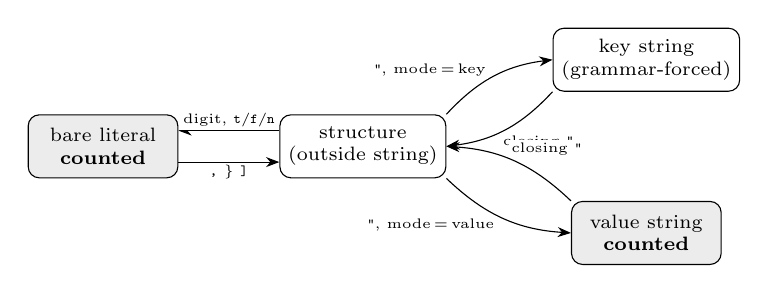
\begin{tikzpicture}[>=Stealth,
  st/.style={draw,rounded corners,align=center,font=\scriptsize,inner sep=3pt,minimum width=19mm,minimum height=8mm},
  cnt/.style={st,fill=gray!15},
  lbl/.style={font=\tiny,align=center,fill=white,inner sep=1pt}]
\node[st] (S) at (0,0) {structure \\ (outside string)};
\node[st] (K) at (3.6,1.1) {key string \\ (grammar-forced)};
\node[cnt] (V) at (3.6,-1.1) {value string \\ \textbf{counted}};
\node[cnt] (L) at (-3.3,0) {bare literal \\ \textbf{counted}};
\draw[->] (S.north east) to[bend left=20] node[lbl,pos=0.45,above left]{\texttt{"}, mode\,=\,key} (K.west);
\draw[->] (K.south west) to[bend left=20] node[lbl,pos=0.55,below right]{closing \texttt{"}} (S.east);
\draw[->] (S.south east) to[bend right=20] node[lbl,pos=0.45,below left]{\texttt{"}, mode\,=\,value} (V.west);
\draw[->] (V.north west) to[bend right=20] node[lbl,pos=0.55,above right]{closing \texttt{"}} (S.east);
\draw[->] ([yshift=2mm]S.west) -- node[lbl,above]{digit, \texttt{t}/\texttt{f}/\texttt{n}} ([yshift=2mm]L.east);
\draw[->] ([yshift=-2mm]L.east) -- node[lbl,below]{\texttt{,} \texttt{\}} \texttt{]}} ([yshift=-2mm]S.west);
\end{tikzpicture}
\caption{The \emph{JsonPos} tracker. Only tokens that land in the two shaded states contribute surprisal; keys and punctuation, which the grammar forces, are ignored. Within the structure state, \texttt{\{} pushes an object and sets mode\,=\,key, \texttt{[} pushes an array and sets mode\,=\,value, \texttt{:} sets mode\,=\,value, \texttt{,} sets mode\,=\,key inside an object and value inside an array, and \texttt{\}}/\texttt{]} pop. Backslash escapes inside strings are consumed without leaving the string state.}
\label{fig:jsonpos}
\end{figure}

\subsection{Calibrating the Confidence Signal}
\label{sec:calibration}

Raw confidence signals are miscalibrated~\cite{guo}, and the surprisal scale is model-, prompt- and schema-specific, so $s_{\max}$ cannot be set by hand. We obtain labels by a \emph{shadow-labeling} pass: each payload of a labeled sample is run through the edge model in a non-aborting mode that records the full value-token surprisal trace. The threshold is the empirical quantile of the training-split signal that hits a target escalation rate, applied unchanged to held-out data. The quantile need not be attainable: with the conventions in context, 87\% of extractions have no measurable surprisal at any value token (below $10^{-4}$\,nats, i.e.\ $p>0.9999$), the target quantile falls inside that tie, and the fitted threshold is zero. The guard then reduces to a rule with no free parameter---\emph{escalate on any measurable hesitation}---and its escalation rate is whatever fraction of traffic the model hesitates on. Where a probability is wanted rather than a decision, isotonic regression~\cite{barlow1972,zadrozny} fits a monotone map from signal to $P(\text{correct})$ and converges at the cube-root rate~\cite{zhang2002}; on a few hundred pairs it did not beat a constant base rate on held-out data, so we treat it as optional. In deployment the only label available is a frontier model's adjudication, so the label-free procedure rests on that judge's fidelity, which Section~\ref{sec:calib} measures against ground truth that does not come from a model.

\subsection{Deterministic Derivation Outside the Quantized Model}
\label{sec:derive}

A small quantized model is unreliable at arithmetic and multi-signal boolean logic, and \texttt{guided\_json} guarantees only that such a field \emph{parses}, not that it is \emph{correct}. We therefore restrict the model to extracting primitives it can read directly off the text and compute every derived field in code. For property audits, the model extracts current and previous values and the cohort baseline; code computes the percentage increase and the discrepancy flag. For telemetry, the model classifies individual stress markers; code computes their count and the ``requires deep diagnostic'' conjunction.

The principle has a second benefit: it makes the schema itself auditable. A production telemetry record reading ``pitch spike +3.1$\sigma$\ldots rigid contraction\ldots multiple stress models triggering simultaneously'' exposed a defect in our first schema, which enumerated acoustic, gaze-duration and off-screen primitives but no posture primitive. The model extracted what it was asked for, the code counted one marker, and \texttt{requires\_deep\_diagnostic} derived to \emph{false}---a valid, schema-conformant, wrong answer that silently dropped the posture signal. Adding a \texttt{posture\_rigid} primitive (extracted, not inferred) raised the count to two and corrected the derivation. Had the conjunction been delegated to the model, the omission would have been a model error with no code path to inspect; because it lived in code, it was a reviewable schema bug. The failure was invisible at the schema level precisely because the output remained valid JSON throughout.

\section{Empirical Results and Scaling Benchmarks}
\label{sec:results}

\subsection{Experimental Setup}
\label{sec:setup}

\paragraph{Host} All results in this section were measured on 20~July~2026 on a single dedicated bare-metal host (Cherry Servers, Stockholm): an AMD Ryzen~9~9950X (Zen~5, 16 physical cores / 32 threads, 186\,GiB RAM, one NUMA node), Ubuntu~24.04.4 LTS, kernel 6.17.0 (EEVDF scheduler). The intervention experiments of Section~\ref{sec:mitigation} were run on 30~September~2026 on a second dedicated host of the same model and provider (Ubuntu~24.04.5, kernel 6.8.0, Node.js~24.21.0; identical CPU, memory, L3 map, runtime version and model checksum), quiesced by the same procedure; its provenance record is in the artifact alongside the first. Both were dedicated bare-metal instances, which isolates the measurements from hypervisor-induced scheduling noise and steal time; bare-metal execution was verified rather than assumed---\texttt{systemd-detect-virt} reports \textsc{none} and no hypervisor CPU flag is present---because a virtualized topology would make core pinning meaningless. Two hardware properties govern the results. First, the processor exposes AVX-512 with VNNI (\texttt{avx512\_vnni}, \texttt{avx\_vnni}), so INT8 kernels are hardware-accelerated. Second, its 64\,MiB of L3 is provisioned as \emph{two} 32\,MiB instances (one per core-complex die, CCD): logical CPUs 0--7 and 16--23 share one domain and 8--15 and 24--31 the other. CPU frequency scaling and boost were left at the distribution defaults; Section~\ref{sec:threats} discusses the resulting confound.

\paragraph{Software and workload} The routing stage embeds each record with \texttt{all-MiniLM-L6-v2}~\cite{minilm,sbert} quantized to INT8 (22.97\,MB; SHA-256 \texttt{afdb6f1a\ldots bdb1}), executed via the native \texttt{onnxruntime-node} binding, version 1.27.0 as resolved by the lockfile, under Node.js~24.18.0 with \texttt{UV\_THREADPOOL\_SIZE}=4 per worker. The broker was Redis~7.0.15 on a dedicated port. \textbf{The scaling experiments isolate the routing stage.} Payloads were short synthetic records (${\approx}$5 tokens, ``\texttt{classify this record $n$}''), the routing threshold was set so that no record escalated, and egress was disabled; the LLM inference stages were therefore not exercised, and every throughput figure below is the throughput of the embedding-and-routing stage in front of them. The guard and calibration results of Section~\ref{sec:calib} come from a separate run against a vLLM server and are described there.

\paragraph{Pinning} Pinned workers were bound with \texttt{taskset} to one logical CPU per physical core (the SMT sibling was left idle), in ascending core order, with \texttt{intraOpNumThreads}=1. Unpinned workers had no affinity mask and could be scheduled on all 32 logical CPUs. The load generator and Redis were pinned together to core~15, on CCD1.

\paragraph{Protocol} Table~\ref{tab:inventory} lists the sampling design of every experiment; they are not uniform, and each table's caption repeats its own $n$ and duration. Confidence intervals are Student-$t$ across independent trials ($t_{4}{=}2.776$ for $n{=}5$, $t_{2}{=}4.303$ for $n{=}3$). Throughput trials ran open-loop at an offered load far above capacity. To obtain an idle host we froze an in-progress RAID1 resync, masked the \texttt{apt-daily} timers, disabled the distribution's Redis unit, and lowered \texttt{kernel.perf\_event\_paranoid} from 4 to 1 for profiling. We record these interventions explicitly, since ``benchmarked on an idle host'' is not a meaningful claim without stating what was silenced to achieve it. The suite requires no network once the model is cached, which we verified by re-running a $W{=}2$ trial under a full egress \texttt{DROP} rule: 4{,}499\,req/s against a networked 4{,}470\,req/s, a 0.6\% difference.

\begin{table}[t]
\caption{Experiment inventory}
\label{tab:inventory}
\centering\footnotesize\setlength{\tabcolsep}{3pt}
\begin{tabular}{@{}llccr@{}}
\toprule
Experiment & Reported in & $n$ & Trial & Load (req/s) \\
\midrule
Pinned vs.\ unpinned sweep & Tab.~\ref{tab:pinunpin},~\ref{tab:marginal}; Fig.~\ref{fig:scaling},~\ref{fig:percore} & 5 & 60\,s & 50k \\
Mechanism, pinned & Tab.~\ref{tab:mech} & 3 & 60\,s & 50k \\
Mechanism, unpinned & Tab.~\ref{tab:mech} & 1 & 90\,s & 50k \\
Spin-wait test (host 2) & Tab.~\ref{tab:intervention}a & 5 & 60\,s & 50k \\
$2\times2$ ablation (host 2) & Tab.~\ref{tab:intervention}b & 5 & 60\,s & 50k \\
Pool-size sweep (host 2) & Tab.~\ref{tab:intervention}c & 5 & 60\,s & 50k \\
Core placement & Tab.~\ref{tab:placement} & 3 & 45\,s & 50k \\
Latency vs.\ load & Tab.~\ref{tab:latency} & 2 & 45\,s & 1.4k--14k \\
Harness ceiling (hash) & \S\ref{sec:harness} & 3 & 20\,s & 200k \\
Air-gap check ($W{=}2$) & \S\ref{sec:setup} & 1 & 30\,s & 50k \\
Guard calibration & Tab.~\ref{tab:calib} & 500 & --- & --- \\
\bottomrule
\end{tabular}
\\[2pt]\footnotesize Throughput runs are open-loop at the stated offered load; $n$ is independent trials (payloads for the calibration row).
\end{table}

\subsection{Harness Validity}
\label{sec:harness}

A throughput benchmark is only meaningful while the measurement apparatus is not itself the bottleneck. We therefore first characterized the harness in isolation by replacing the embedding stage with a deterministic hash, leaving the broker, batching and egress path intact. Plumbing-only throughput ranged from 106{,}312\,req/s at two workers to 91{,}785\,req/s at fourteen, with the load generator never exceeding 41\% of one core and Redis never exceeding 27\%.

Peak real-mode throughput measured anywhere in this paper is 21{,}803\,req/s, a $4.2\times$ margin below the harness ceiling at the same worker count. Across every trial reported below, load-generator CPU never exceeded 24\% and Redis never exceeded 18.4\%; both are recorded per trial alongside throughput, so the claim that no data point was harness-limited is auditable rather than asserted. The load generator is round-trip-bound rather than CPU-bound: it dispatches a pipelined batch every 20\,ms and each iteration also costs a broker round trip, which caps achievable offered load below what its CPU utilization would suggest and is the reason the latency sweep of Section~\ref{sec:latency} does not reach $\rho \to 1$.

\subsection{The Unpinned Pathology}
\label{sec:unpinned}

Table~\ref{tab:pinunpin} and Fig.~\ref{fig:scaling} present the central result. Under the default configuration---ONNX Runtime sizing its intra-op pool to the logical-CPU count, with no OS-level affinity---the fleet does not merely scale sub-linearly. It scales \emph{negatively}: aggregate throughput \emph{falls} monotonically as workers are added, from 4{,}123\,req/s at a single worker to 1{,}381\,req/s at fourteen, converging toward a floor that is largely independent of fleet size. The pinned configuration over the same range rises from 2{,}285 to 21{,}803\,req/s.

\begin{table}[t]
\caption{Pinned versus unpinned throughput ($n{=}5$, 60\,s trials, mean $\pm$ 95\% $t$-interval)}
\label{tab:pinunpin}
\centering\small\setlength{\tabcolsep}{3pt}
\begin{tabular}{@{}crrr@{}}
\toprule
$W$ & Pinned (req/s) & Unpinned (req/s) & Ratio \\
\midrule
1  & 2{,}285 $\pm$14  & \textbf{4{,}123 $\pm$309} & \textbf{0.55}$\times$ \\
2  & 4{,}470 $\pm$15  & 1{,}981 $\pm$18  & 2.26$\times$ \\
4  & 8{,}618 $\pm$12  & 1{,}721 $\pm$51  & 5.01$\times$ \\
6  & 12{,}123 $\pm$41 & 1{,}566 $\pm$9   & 7.74$\times$ \\
8  & 14{,}124 $\pm$54 & 1{,}514 $\pm$49  & 9.33$\times$ \\
10 & 17{,}862 $\pm$14 & 1{,}417 $\pm$67  & 12.60$\times$ \\
12 & 20{,}544 $\pm$147& 1{,}397 $\pm$15  & 14.71$\times$ \\
14 & \textbf{21{,}803 $\pm$193} & \textbf{1{,}381 $\pm$13} & \textbf{15.79}$\times$ \\
\bottomrule
\end{tabular}
\\[2pt]\footnotesize Ratio $>1$ favors pinning. At $W{=}1$ the \emph{unpinned}
configuration wins by $1.80\times$.
\end{table}

\begin{figure}[t]
\centering
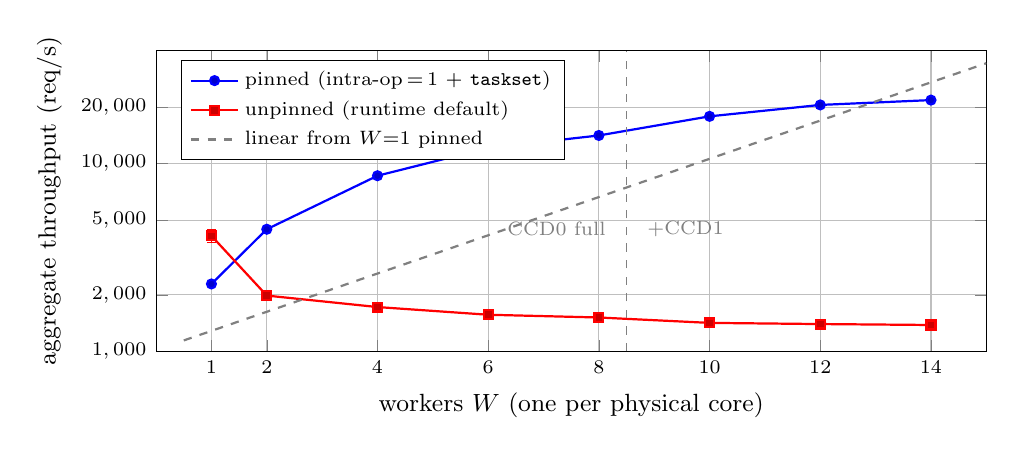
\begin{tikzpicture}
\begin{semilogyaxis}[width=\columnwidth,height=5.4cm,
  xlabel={workers $W$ (one per physical core)},ylabel={aggregate throughput (req/s)},
  xmin=0,xmax=15,ymin=1000,ymax=40000,xtick={1,2,4,6,8,10,12,14},
  ytick={1000,2000,5000,10000,20000},log ticks with fixed point,
  yticklabel style={/pgf/number format/.cd,fixed,precision=0,1000 sep={,}},
  grid=major,tick label style={font=\scriptsize},label style={font=\small},
  legend pos=north west,legend style={font=\scriptsize,cells={anchor=west}},
  every axis plot/.append style={thick}]
\addplot+[mark=*,mark size=1.6pt,error bars/.cd,y dir=both,y explicit] coordinates {
 (1,2285)+-(0,14) (2,4470)+-(0,15) (4,8618)+-(0,12) (6,12123)+-(0,41) (8,14124)+-(0,54) (10,17862)+-(0,14) (12,20544)+-(0,147) (14,21803)+-(0,193)};
\addlegendentry{pinned (intra-op\,=\,1 + \texttt{taskset})}
\addplot+[mark=square*,mark size=1.6pt,error bars/.cd,y dir=both,y explicit] coordinates {
 (1,4123)+-(0,309) (2,1981)+-(0,18) (4,1721)+-(0,51) (6,1566)+-(0,9) (8,1514)+-(0,49) (10,1417)+-(0,67) (12,1397)+-(0,15) (14,1381)+-(0,13)};
\addlegendentry{unpinned (runtime default)}
\addplot[gray,dashed,domain=0.5:15,samples=2] {2285*x};
\addlegendentry{linear from $W{=}1$ pinned}
\draw[gray,dashed] (axis cs:8.5,1000) -- (axis cs:8.5,40000);
\node[gray,font=\scriptsize,anchor=east] at (axis cs:8.3,4500) {CCD0 full};
\node[gray,font=\scriptsize,anchor=west] at (axis cs:8.7,4500) {$+$CCD1};
\end{semilogyaxis}
\end{tikzpicture}
\caption{Aggregate throughput versus fleet size (log scale; $n{=}5$, error bars are 95\% $t$-intervals and are mostly smaller than the markers). The unpinned default wins at $W{=}1$ and loses everywhere else. Workers 1--8 occupy CCD0; worker 9 is the first on CCD1.}
\label{fig:scaling}
\end{figure}

The crossover sits between one and two workers, and it is the practically important feature of the table. A single unpinned worker \emph{outperforms} a pinned one by $1.80\times$, because it commandeers all sixteen cores for one matrix multiplication. Adding a second worker halves absolute throughput, while the pinned fleet nearly doubles. The configuration that wins every single-process microbenchmark therefore loses by $15.8\times$ at fleet scale---which is precisely why the defect survives into deployment: practitioners select on the isolated measurement, and the isolated measurement is unambiguous and wrong.

An unpinned worker carries 42 threads against 11 when pinned, so the fourteen-worker fleet presents roughly 588 threads to 16 physical cores. Every trial nonetheless completed and every worker cleared its readiness gate: the pathology is throughput collapse, not initialization failure. Variance is also informative---the unpinned $W{=}1$ interval ($\pm$309) is an order of magnitude wider than at $W{=}2$ ($\pm$18), consistent with a single pool being scheduled opportunistically across idle cores, then settling into deterministic contention once the machine is saturated.

\subsection{Pinned Scaling and the L3 Discontinuity}
\label{sec:l3}

Pinned scaling is near-linear only within a bounded regime, and its marginal efficiency is \emph{not monotonic} (Table~\ref{tab:marginal}, Fig.~\ref{fig:percore}). We define the step efficiency from $W_1$ to $W_2$ workers as the measured throughput gain divided by the ideal gain $W_2/W_1$. It holds at 94--98\% while workers share a single L3 domain, decays to 87.4\% as that domain saturates at eight workers, and then \emph{recovers} to 101.2\% at the step where the fleet first spills onto the second chiplet: per-core throughput \emph{rises} across that boundary, from 1{,}765 to 1{,}786\,req/s. The recovery is relative to the preceding saturated step, not to $W{=}1$; per-core throughput at $W{=}10$ is 78\% of its $W{=}1$ value, and overall efficiency across the full $1\rightarrow14$ range is 68.2\%. An unqualified claim of near-linear scaling would not survive scrutiny at fleet scale.

\begin{table}[t]
\caption{Marginal scaling efficiency, pinned (from Table~\ref{tab:pinunpin}, $n{=}5$)}
\label{tab:marginal}
\centering\small\setlength{\tabcolsep}{4pt}
\begin{tabular}{@{}lccl@{}}
\toprule
Step & Gain & Efficiency & L3 domain \\
\midrule
$1\rightarrow2$   & 1.956$\times$ & 97.8\%  & CCD0 \\
$2\rightarrow4$   & 1.928$\times$ & 96.4\%  & CCD0 \\
$4\rightarrow6$   & 1.407$\times$ & 93.8\%  & CCD0 \\
$6\rightarrow8$   & 1.165$\times$ & 87.4\%  & CCD0 saturating \\
$\mathbf{8\rightarrow10}$ & \textbf{1.265}$\times$ & \textbf{101.2\%} & \textbf{crosses to CCD1} \\
$10\rightarrow12$ & 1.150$\times$ & 95.8\%  & both \\
$12\rightarrow14$ & 1.061$\times$ & 91.0\%  & both \\
\bottomrule
\end{tabular}
\\[2pt]\footnotesize Efficiency $=$ gain $\div$ ideal gain ($W_2/W_1$).
\end{table}

\begin{figure}[t]
\centering
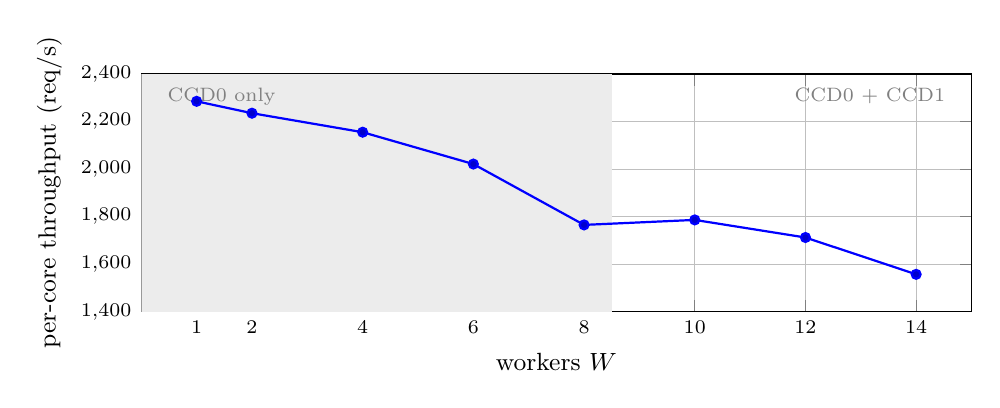
\begin{tikzpicture}
\begin{axis}[width=\columnwidth,height=4.6cm,
  xlabel={workers $W$},ylabel={per-core throughput (req/s)},
  xmin=0,xmax=15,ymin=1400,ymax=2400,xtick={1,2,4,6,8,10,12,14},
  grid=major,tick label style={font=\scriptsize},label style={font=\small},
  every axis plot/.append style={thick}]
\fill[gray!15] (axis cs:0,1400) rectangle (axis cs:8.5,2400);
\node[gray,font=\scriptsize,anchor=north west] at (axis cs:0.3,2380) {CCD0 only};
\node[gray,font=\scriptsize,anchor=north east] at (axis cs:14.7,2380) {CCD0 + CCD1};
\addplot+[mark=*,mark size=1.6pt] coordinates {(1,2285) (2,2235) (4,2155) (6,2021) (8,1765) (10,1786) (12,1712) (14,1557)};
\end{axis}
\end{tikzpicture}
\caption{Pinned per-core throughput (aggregate $\div W$). It declines as one L3 domain fills and rises at $W{=}10$, the first point at which workers occupy both chiplets.}
\label{fig:percore}
\end{figure}

Operating-system telemetry supplies a mechanism. Inspection of \texttt{/proc/\textit{pid}/maps} shows \emph{no} file-backed mapping of the quantized model: the weights are read into anonymous memory, so each worker holds a private copy of the 23\,MB INT8 model rather than sharing physical pages through the page cache (each worker's total \texttt{Private\_Dirty} is 232\,MB, of which the model is one part). Eight workers co-resident on one 32\,MiB L3 domain therefore stream an aggregate weight working set of roughly 184\,MB through it, on top of activations. The recovery at the boundary is the consequence: crossing to the second chiplet does not add cores so much as it adds a second 32\,MiB cache domain. We have not measured L3 miss rates directly, so this is an inference from topology and memory maps; the placement experiment below tests it.

\subsection{Core Placement Is Worth 16.7\%}
\label{sec:placement}

If the effect above is attributable to cache capacity rather than core count, it should be recoverable by placement alone. Table~\ref{tab:placement} isolates the two candidate factors at fixed worker count.

\begin{table}[t]
\caption{Core-placement matrix ($n{=}3$, 45\,s trials, mean $\pm$ 95\% $t$-interval); infra pinned to core 15 (CCD1)}
\label{tab:placement}
\centering\small\setlength{\tabcolsep}{4pt}
\begin{tabular}{@{}llcr@{}}
\toprule
Run & Worker cores & L3 domains & req/s \\
\midrule
C1 & 0--3          & 1 (CCD0) & 8{,}656 $\pm$81 \\
C2 & 8--11         & 1 (CCD1)$^{\dagger}$ & 8{,}346 $\pm$82 \\
A  & 0--7          & 1 (packed) & 14{,}183 $\pm$91 \\
\textbf{B} & \textbf{0--3, 8--11} & \textbf{2 (split)} & \textbf{16{,}556 $\pm$106} \\
\bottomrule
\end{tabular}
\\[2pt]\footnotesize $^{\dagger}$C2 shares CCD1 with the pinned load generator and
broker. C1 and A reproduce the corresponding points of Table~\ref{tab:pinunpin}
to within 0.5\%.
\end{table}

Runs A and B use identical worker and core counts and differ only in which chiplets those cores belong to; splitting the fleet across both L3 domains yields \textbf{16.7\% higher throughput at zero hardware cost}, a difference of more than twenty interval half-widths. Measured against two independent four-worker groups ($2\times$C1 $=$ 17{,}312\,req/s), the packed arrangement achieves 81.9\% of that ideal and the split arrangement 95.6\%.

The comparison of C1 against C2 bounds the competing explanation. Placing workers on the \emph{same} chiplet as the broker and load generator---minimizing cross-fabric distance---was 3.6\% \emph{slower}, not faster, because the infrastructure processes consume L3 the workers need. Inter-chiplet distance to the broker is thus a minor and, in this configuration, adverse term; cache capacity dominates. The practical consequence is that the naive ascending core assignment of Table~\ref{tab:pinunpin} leaves throughput unclaimed at intermediate fleet sizes (16.7\% at $W{=}8$), and that scheduling policy for CPU inference fleets on chiplet processors should be L3-aware rather than core-count-aware.

\subsection{Latency versus Offered Load}
\label{sec:latency}

The saturation runs above measure throughput correctly and latency not at all: at an offered load $3.5\times$ the eight-worker capacity, time-to-answer is dominated by queue backlog and $p99$ approaches four seconds. To characterize latency we therefore held offered load constant at a series of sub-capacity rates against a fixed eight-worker pinned fleet ($\mu = 14{,}124$\,req/s), so that the queue does not diverge (Table~\ref{tab:latency}).

\begin{table}[t]
\caption{Latency versus offered load, $W{=}8$ pinned ($n{=}2$, 45\,s trials, means)}
\label{tab:latency}
\centering\small\setlength{\tabcolsep}{3.5pt}
\begin{tabular}{@{}rrcrrr@{}}
\toprule
Offered & Achieved & $\rho$ & $p50$ & $p95$ & $p99$ \\
(req/s) & (req/s) & & (ms) & (ms) & (ms) \\
\midrule
1{,}400  & 1{,}296  & 0.09 & 15.0 & 27.5 & 28.5 \\
2{,}800  & 2{,}581  & 0.18 & 16.0 & 28.0 & 29.0 \\
5{,}600  & 5{,}112  & 0.36 & 18.0 & 30.5 & 34.0 \\
8{,}500  & 7{,}720  & 0.55 & 20.0 & 34.5 & 59.0 \\
11{,}300 & 10{,}180 & 0.72 & 25.0 & 41.0 & 129.0 \\
12{,}700 & 11{,}405 & 0.81 & 30.0 & 46.5 & 164.0 \\
13{,}400 & 11{,}914 & 0.84 & 33.0 & 58.0 & 184.5 \\
14{,}000 & 12{,}467 & \textbf{0.88} & \textbf{36.5} & \textbf{62.5} & \textbf{200.0} \\
\bottomrule
\end{tabular}
\\[2pt]\footnotesize $\rho$ $=$ achieved $\div$ $\mu$. Percentiles are computed per trial over completed requests and averaged; the two trials agree to within 4\,ms at every cell.
\end{table}

The measurements reproduce the qualitative prediction of Eq.~(\ref{eq:pk}): the tail diverges far ahead of the median. Across the sweep the median grows $2.4\times$ (15.0 to 36.5\,ms) while $p99$ grows $7.0\times$ (28.5 to 200\,ms), with the $p99$ knee appearing near $\rho\approx0.55$ while $p50$ is still almost flat. At low utilization the distribution is tight---$p95$ and $p99$ differ by 1\,ms at $\rho=0.09$---and it is that separation, not the median, which widens as capacity is approached. An SLA expressed on mean latency would report a system in good health well past the point at which its tail has begun to fail.

Two limitations are visible in the table. Achieved throughput falls short of the nominal offered rate by 7--11\% at every row, including rates far below capacity; this is a property of the generator's timer-driven dispatch loop, which accumulates drift on each iteration's broker round trip, and not of the system under test. We therefore report achieved rather than nominal load throughout. Second, realized utilization consequently reached $\rho\approx0.88$ rather than 0.99. Driving the system closer to $\rho\rightarrow1$ requires a generator with an absolute dispatch schedule; the divergence we report is real and correctly ordered, but the asymptotic region immediately below saturation remains unmeasured.

\subsection{Guard Evaluation}
\label{sec:calib}

\paragraph{Stack} The guard experiments used a separate serving path. The edge model is Qwen3-8B quantized with AWQ~\cite{awq} to 4 bits (group size 128; the official \texttt{Qwen/Qwen3-8B-AWQ} release), served by vLLM~0.9.2 with the \texttt{xgrammar} guided-decoding backend and \texttt{guided\_json} constraints on a single NVIDIA RTX~3090 (24\,GB; rented hosts whose GPU is attached at PCIe~4.0 $\times$16, verified by link state and a measured 18.7\,GiB/s host-to-device copy). The model is queried at temperature zero through the completions endpoint with its chat-turn format applied and reasoning output disabled. Model identities, the prompt format and the in-context examples are fixed in the artifact's \texttt{src/models.mjs} and schema registry, and the worker and the benchmark build the prompt with the same function. The masking probe of Section~\ref{sec:conflict} returned \textsc{post-mask} ($H=0.049$\,nats at the first structural token) on this stack.

\paragraph{Corpora} Ground truth is \emph{constructed rather than inferred}. For each record the field values are sampled in code from a seeded generator; a language model is used only as a writer that verbalizes those facts in one of five styles (clean, shorthand, distractor, negation, reordered). Because a writer can be unfaithful, every text is then checked mechanically, with no model in the loop, for whether the constructed truth can be read off it: each stated number, verbatim phrase and negation is matched against the text, and absent fields are checked to be absent. Texts that fail are regenerated. We used two such corpora, each half property-audit and half telemetry. A 500-record \emph{exploratory} corpus served to diagnose the guard, choose its statistic and schema rules (Section~\ref{sec:jsonpos}) and explore generation settings. A fresh 2{,}000-record \emph{confirmation} corpus, generated with a new seed after every design choice and both in-context examples were frozen, is the only one whose results we report as findings; 349 of its first drafts (17\%) failed the faithfulness check and were regenerated, and two fell back to a deterministic template. Both corpora, the generator and all per-record traces are in the artifact; neither contains personal data.

\paragraph{Protocol} The confirmation analysis was committed to the artifact repository before the confirmation data were collected. It fixes three arms---zero, one and two in-context examples at temperature zero---the decision statistic (mean surprisal over all value tokens), a 70/30 split stratified by workload, a threshold fit on the 1{,}400 training records at a 20\% escalation target and applied unchanged to the 600 held-out records, the metrics, and the tests. An extraction is correct if every decision primitive of its schema matches the constructed truth (numbers within 0.05; lists as sets). A \emph{silent error} is an incorrect extraction that the guard keeps local, counted as a share of all records. Intervals are Wilson 95\%~\cite{wilson1927}; differences are paired bootstraps over held-out records (10{,}000 resamples).

\paragraph{First-order lever: prompt conventions} Table~\ref{tab:calib}a reports the edge model alone. Zero-shot it is correct on 78.3\% of held-out records, and its errors are reading errors rather than arithmetic ones: boolean markers set without support (\texttt{posture\_rigid} 47, \texttt{baseline\_nominal} 25, \texttt{gaze\_offscreen} 22), list items mis-copied or invented (31), stated numbers set to \texttt{null} (22). One in-context example lifts accuracy to 91.5\% ($+13.2$ points, interval $+9.7$ to $+16.8$) and two lift it to 97.0\% ($+18.7$, $+15.3$ to $+22.0$); the second example adds $+5.5$ ($+3.7$ to $+7.3$). The effect is concentrated where the conventions matter: telemetry rises from 67.3\% to 100\% of 300 held-out records, and the styles the zero-shot model finds hardest, distractor and reordered text (67\% correct across the corpus), reach 95\%. With two examples every remaining error is a list-item mismatch.

\paragraph{Second-order filter: the guard} Table~\ref{tab:calib}b reports the guard on top of each arm. Its signal separates errors from correct extractions with a held-out AUROC of 0.79 zero-shot and 0.85--0.90 with examples. Zero-shot, at the fitted threshold of 0.021\,nats it escalates 21.0\% of records and catches 49.2\% of 130 errors, leaving 11.0\% of all records silently wrong against 21.7\% with no guard. With two examples the fitted threshold is zero (Section~\ref{sec:calibration}): the guard escalates the 13.7\% of records on which the model shows any hesitation, catches 14 of the 18 errors, and leaves 0.7\% silently wrong against 3.0\% with no guard ($-2.3$ points, interval $-3.7$ to $-1.2$). The guard's contribution is statistically clear in every arm (Table~\ref{tab:calib}c) and shrinks as the prompt improves, which is what second-order means: it removes 10.7 points of silent error from a weak prompt and 2.3 from a good one. With the guard in place, one and two examples are indistinguishable in silent-error rate (1.0\% and 0.7\%), but two examples reach it while escalating 13.7\% of traffic rather than 22.2\%; the pre-registered rule selects the two-example prompt.

\begin{table}[t]
\caption{Confirmation experiment: held-out split ($n{=}600$) of 2{,}000 fresh records; thresholds fit on the 1{,}400 training records}
\label{tab:calib}
\centering\footnotesize\setlength{\tabcolsep}{2.5pt}
\begin{tabular}{@{}lcccc@{}}
\toprule
\multicolumn{5}{@{}l}{\textit{(a) Edge model alone}} \\
Prompt & Accuracy & Errors & Property & Telemetry \\
\midrule
0-shot & 78.3 (74.9--81.4) & 130 & 89.3 & 67.3 \\
1-shot & 91.5 (89.0--93.5) & 51 & 84.3 & 98.7 \\
\textbf{2-shot} & \textbf{97.0 (95.3--98.1)} & \textbf{18} & 94.0 & 100.0 \\
\midrule
\multicolumn{5}{@{}l}{\textit{(b) With the value-surprisal guard}} \\
Prompt & AUROC & Escalated & Error recall & Silent errors \\
\midrule
0-shot & 0.794 & 21.0 & 49.2 (40.8--57.7) & 11.0 (8.7--13.8) \\
1-shot & 0.896 & 22.2 & 88.2 (76.6--94.5) & 1.0 (0.5--2.2) \\
\textbf{2-shot} & 0.851 & \textbf{13.7} & 77.8 (54.8--91.0) & \textbf{0.7 (0.3--1.7)} \\
\midrule
\multicolumn{5}{@{}l}{\textit{(c) Paired differences, percentage points (95\% interval)}} \\
\midrule
\multicolumn{3}{@{}l}{Accuracy, 2-shot $-$ 0-shot} & \multicolumn{2}{r@{}}{$+18.7$ ($+15.3$, $+22.0$)} \\
\multicolumn{3}{@{}l}{Accuracy, 2-shot $-$ 1-shot} & \multicolumn{2}{r@{}}{$+5.5$ ($+3.7$, $+7.3$)} \\
\multicolumn{3}{@{}l}{Silent errors, guard $-$ no guard, 0-shot} & \multicolumn{2}{r@{}}{$-10.7$ ($-13.2$, $-8.3$)} \\
\multicolumn{3}{@{}l}{Silent errors, guard $-$ no guard, 2-shot} & \multicolumn{2}{r@{}}{$-2.3$ ($-3.7$, $-1.2$)} \\
\multicolumn{3}{@{}l}{Silent errors with guard, 2-shot $-$ 0-shot} & \multicolumn{2}{r@{}}{$-10.3$ ($-12.8$, $-7.8$)} \\
\multicolumn{3}{@{}l}{Silent errors with guard, 2-shot $-$ 1-shot} & \multicolumn{2}{r@{}}{$-0.3$ ($-1.0$, $+0.3$)} \\
\bottomrule
\end{tabular}
\\[2pt]\footnotesize Percentages; Wilson 95\% intervals in (a) and (b). Silent errors: incorrect and kept local, as a share of all 600 records; without a guard they equal the error rate (21.7\%, 8.5\%, 3.0\%).
\end{table}

\paragraph{What did not help, and what does not work} Three further observations come from the exploratory corpus and from descriptive analysis of the confirmation traces, and carry less weight than the table. First, softening the output distribution does not make errors more detectable: across temperatures 0 to 0.5 the zero-shot model's accuracy (74.2\% to 73.0\%), its silent-error rate (13.3\% at every setting) and the reported log-probabilities (within 0.0013\,nats on token-identical records) were unchanged. Second, the windowed statistic of our original design is at chance on the property-audit workload in every arm of the confirmation run (held-out AUROC 0.50, against 0.65--0.85 for the mean over all value tokens), because the leading multi-digit value fills the window. Third, the frontier judge that a label-free deployment would rely on agreed with constructed truth on 96.4\% of the exploratory records (CI 94.4--97.7), so shadow labeling carries a label-noise floor of roughly 3\%.

These results bound what each mechanism can be asked to do. The surprisal signal is real, and a grammar-masked entropy guard would have seen nothing at all. But the guard alone, on a weak prompt, leaves one record in nine silently wrong; it is the prompt that brings the error rate down by an order of magnitude, and the guard that then removes about three quarters of what is left at a modest escalation cost. The residue---list items copied wrongly with full confidence---is invisible to any confidence-based check and needs a different one. We also note that edge latency through our tunnel to the rented host was 1.1--1.9\,s per object, so the in-stream deadline of the production path was not exercised.

\section{Threats to Validity}
\label{sec:threats}

\begin{enumerate}
\item \emph{Scope of the throughput results.} Every throughput and latency figure measures the CPU-resident embedding-and-routing stage with short synthetic payloads and no LLM inference in the loop (Section~\ref{sec:setup}). The oversubscription pathology is a property of that stage and would apply to any fleet of ONNX Runtime sessions; absolute figures for a full cascade will be lower and workload-dependent.
\item \emph{Two-variable treatment.} The scaling results of Section~\ref{sec:results} use the combined ``pinned'' treatment. The ablation of Table~\ref{tab:intervention}b shows the \texttt{taskset} component contributes $-0.8\%$, so those results can be read as results for a single-thread pool; they were not, however, re-measured without affinity beyond $W{=}8$ and $14$.
\item \emph{Mechanism attribution.} Spin-wait contention is demonstrated by intervention (Table~\ref{tab:intervention}a), not by symbol: the dominant call site of Table~\ref{tab:mech} remains unnamed because the distributed \texttt{libonnxruntime.so} carries no symbols. The loss that disabling spinning does not recover is measured directly in Table~\ref{tab:intervention}c at $W{=}8$ (at most 19\% at the default pool size) but not at $W{=}14$, where it is larger; the sweep also exposed a 12\% run-to-run variation in the large-pool, non-spinning configuration that the single-thread configurations do not show. The unpinned telemetry of Table~\ref{tab:mech} rests on a single 90\,s trial; the intervention experiments were run on a second host of the same model, whose reference arm reproduced the first host within 1.3\%.
\item \emph{Frequency scaling.} Boost clocks were not disabled and per-core frequency was not logged. Zen~5 boost depends on the number of active cores, which is a confound for the single-worker inversion and for per-step efficiency; the sign and magnitude of the 15.8$\times$ effect are far outside anything frequency alone can produce, but the efficiency percentages in Table~\ref{tab:marginal} should be read with this in mind.
\item \emph{L3 attribution.} The cache explanation of the chiplet discontinuity is inferred from topology, memory maps and the placement experiment; L3 miss rates were not measured.
\item \emph{Co-location and generator ceiling.} The load generator and broker ran on a core of the same host (an effect Table~\ref{tab:placement} measures at 3.6\%), and the generator's drift capped realized utilization at $\rho\approx0.88$. An external, absolutely scheduled generator is required to close both gaps.
\item \emph{Single microarchitecture.} All figures are from one desktop-class Zen~5 part with AVX-512/VNNI and a dual-chiplet L3. We expect the oversubscription pathology on any multi-core host running the same runtime default, but the magnitudes are not portable: parts with a monolithic L3 should not exhibit the discontinuity, parts with more chiplets may exhibit it repeatedly, and cores without VNNI will show lower per-core throughput. Server-class parts and a second vendor remain untested.
\item \emph{Host interventions.} The measured configuration is a deliberately quiesced one (Section~\ref{sec:setup}), not a stock installation.
\item \emph{Guard evaluation scope.} The correctness results rest on one edge model, one serving stack and synthetic text. The confirmation corpus is fresh and its analysis was fixed in advance, but it comes from the same generator as the exploratory corpus on which the in-context examples were designed, so it tests generalization within that distribution, not to production traffic, which is longer and noisier. The writer of the texts and the judge are the same model family, although ground truth is constructed in code, every text is verified mechanically, and judge fidelity is measured against that truth rather than assumed. With two examples only 18 held-out errors remain, so the guard's recall on that arm (77.8\%) has a wide interval, and the surviving error class is one the guard cannot see. A zero threshold means the guard's behavior depends on the resolution at which surprisal is recorded ($10^{-4}$\,nats here). An earlier draft of this paper reported a far more favorable operating point from an internal run whose data were not retained; that result could not be reproduced and is withdrawn.
\item \emph{Delivery semantics.} At-least-once delivery makes idempotent sinks mandatory; only the \texttt{pgvector} sink in the reference implementation is idempotent. Recovery of a crashed consumer's pending entries is implemented but was not exercised in the benchmarks reported here.
\item \emph{Cost model.} Eq.~(\ref{eq:cost}) is an analytical bound; realized savings depend on the workload's true hard-payload rate.
\end{enumerate}

\section{Conclusion and Future Work}

The throughput of an LLM ingestion pipeline is set in its CPU-resident stage, by runtime behavior the application never sees. The dominant lever is not the routing policy but thread discipline: the ONNX Runtime default silently oversubscribes the host, the fleet scales \emph{negatively}, and one intra-op thread per worker yields a $15.8\times$ advantage at fourteen workers on bare-metal x86. That the same default \emph{wins} by $1.8\times$ in single-process isolation is what makes the defect durable in production. Context-switch churn cannot be the cause; the mechanism is the pool's userspace spin-wait, demonstrated by disabling it alone and recovering 81\% of the loss at eight workers, and the remedy is the pool size, not OS affinity, which a factorial ablation shows contributes nothing. Scaling is then bounded by L3 capacity---decaying within a chiplet and recovering across the boundary---so placement policy is worth a further 16.7\% at no hardware cost.

The cascade's correctness fallback is the secondary result. Constrained decoding guarantees parseable output while creating a silent-failure mode that defeats entropy-based guards, and a guard re-pointed at grammar-free value positions recovers a real signal. But the ordering of the levers is the finding: in a pre-registered experiment against constructed ground truth, two in-context examples of the schema's conventions raised the local model's accuracy from 78\% to 97\%, and the guard then removed about three quarters of the residual errors, lowering the silent-error rate from 3.0\% to 0.7\% at a 13.7\% escalation rate. The guard on its own, over a weak prompt, leaves 11\%. Two apparently harmless choices---optional schema fields and a windowed statistic---each reduce it to chance without any visible failure, and the errors that survive are confident ones that no confidence-based check will catch. Keeping derived logic in code removes one further class of valid-but-wrong output and makes the rest auditable.

Future work, in order of leverage: (i)~replication on monolithic-L3 and many-chiplet parts, with L3 miss-rate counters, to establish how far the placement result generalizes; (ii)~repeating the pool-size sweep at $W{=}14$ and across spin-duration settings, with per-trial frequency logging, to characterize the large-pool variation observed in Section~\ref{sec:mitigation}; (iii)~an absolutely scheduled external load generator to reach $\rho\rightarrow1$; (iv)~evaluating the prompt conventions and the guard on production traffic with human-audited labels and on additional edge models, and adding a confidence-independent check for the list-item errors that survive both; and (v)~evaluating hybrid speculative-cascade decoding to combine cost routing with lossless token-level acceleration.

\section*{Ethics and Data Statement}
This research involved no human subjects and no personal data. The throughput benchmarks use synthetic records, and the guard is evaluated on synthetic corpora whose every value is a random draw from a seeded generator (Section~\ref{sec:calib}); the corpora are published with the artifact. The four illustrative payloads that accompany Section~\ref{sec:derive} are pseudonymized.

\section*{Artifact Availability}
The complete source code, deployment manifests, benchmark harness, raw per-trial CSVs for every table, the provenance records of both measurement hosts, and the immutable telemetry and \texttt{perf} captures are available at \url{https://github.com/mosafariuk/edge-cascade}. The synthetic calibration corpus, its generator, the per-record guard traces and the pre-registered analysis script that produces Table~\ref{tab:calib} are included.

\section*{Acknowledgments}
This research received no external funding. The author declares no conflicts of interest.

\begin{thebibliography}{00}
\bibitem{frugalgpt} L.~Chen, M.~Zaharia, and J.~Zou, ``FrugalGPT: How to use large language models while reducing cost and improving performance,'' \emph{Trans. Mach. Learn. Res.}, 2024. arXiv:2305.05176.
\bibitem{leviathan} Y.~Leviathan, M.~Kalman, and Y.~Matias, ``Fast inference from transformers via speculative decoding,'' in \emph{Proc. ICML}, 2023. arXiv:2211.17192.
\bibitem{chensp} C.~Chen \emph{et al.}, ``Accelerating large language model decoding with speculative sampling,'' \emph{arXiv:2302.01318}, 2023.
\bibitem{fastercascades} H.~Narasimhan \emph{et al.}, ``Faster cascades via speculative decoding,'' \emph{arXiv:2405.19261}, 2024.
\bibitem{routellm} I.~Ong \emph{et al.}, ``RouteLLM: Learning to route LLMs with preference data,'' \emph{arXiv:2406.18665}, 2024.
\bibitem{hybridllm} D.~Ding \emph{et al.}, ``Hybrid LLM: Cost-efficient and quality-aware query routing,'' in \emph{Proc. ICLR}, 2024. arXiv:2404.14618.
\bibitem{automix} P.~Aggarwal \emph{et al.}, ``AutoMix: Automatically mixing language models,'' \emph{arXiv:2310.12963}, 2023.
\bibitem{chow1970} C.~K.~Chow, ``On optimum recognition error and reject tradeoff,'' \emph{IEEE Trans. Inf. Theory}, vol.~16, no.~1, pp.~41--46, 1970.
\bibitem{geifman2017} Y.~Geifman and R.~El-Yaniv, ``Selective classification for deep neural networks,'' in \emph{Proc. NeurIPS}, 2017.
\bibitem{vllm} W.~Kwon \emph{et al.}, ``Efficient memory management for large language model serving with PagedAttention,'' in \emph{Proc. SOSP}, 2023. arXiv:2309.06180.
\bibitem{ort_docs} ONNX Runtime Developers, ``ONNX Runtime performance tuning: Threading.'' [Online]. Available: \url{https://onnxruntime.ai/docs/performance/tune-performance/threading.html} (accessed 30 Sep. 2026).
\bibitem{iancu2010} C.~Iancu, S.~Hofmeyr, F.~Blagojevi\'c, and Y.~Zheng, ``Oversubscription on multicore processors,'' in \emph{Proc. IEEE IPDPS}, 2010.
\bibitem{outlines} B.~T.~Willard and R.~Louf, ``Efficient guided generation for large language models,'' \emph{arXiv:2307.09702}, 2023.
\bibitem{xgrammar} Y.~Dong \emph{et al.}, ``XGrammar: Flexible and efficient structured generation engine for large language models,'' \emph{arXiv:2411.15100}, 2024.
\bibitem{sglang} L.~Zheng \emph{et al.}, ``SGLang: Efficient execution of structured language model programs,'' in \emph{Proc. NeurIPS}, 2024. arXiv:2312.07104.
\bibitem{kuhn2023semantic} L.~Kuhn, Y.~Gal, and S.~Farquhar, ``Semantic uncertainty: Linguistic invariances for uncertainty estimation in natural language generation,'' in \emph{Proc. ICLR}, 2023. arXiv:2302.09664.
\bibitem{awq} J.~Lin \emph{et al.}, ``AWQ: Activation-aware weight quantization for LLM compression and acceleration,'' in \emph{Proc. MLSys}, 2024. arXiv:2306.00978.
\bibitem{minilm} W.~Wang \emph{et al.}, ``MiniLM: Deep self-attention distillation for task-agnostic compression of pre-trained transformers,'' in \emph{Proc. NeurIPS}, 2020. arXiv:2002.10957.
\bibitem{sbert} N.~Reimers and I.~Gurevych, ``Sentence-BERT: Sentence embeddings using Siamese BERT-networks,'' in \emph{Proc. EMNLP}, 2019. arXiv:1908.10084.
\bibitem{guo} C.~Guo, G.~Pleiss, Y.~Sun, and K.~Q.~Weinberger, ``On calibration of modern neural networks,'' in \emph{Proc. ICML}, 2017. arXiv:1706.04599.
\bibitem{zadrozny} B.~Zadrozny and C.~Elkan, ``Transforming classifier scores into accurate multiclass probability estimates,'' in \emph{Proc. KDD}, 2002.
\bibitem{barlow1972} R.~E.~Barlow, D.~J.~Bartholomew, J.~M.~Bremner, and H.~D.~Brunk, \emph{Statistical Inference under Order Restrictions}. Wiley, 1972.
\bibitem{zhang2002} C.-H.~Zhang, ``Risk bounds in isotonic regression,'' \emph{Ann. Statist.}, vol.~30, no.~2, pp.~528--555, 2002.
\bibitem{wilson1927} E.~B.~Wilson, ``Probable inference, the law of succession, and statistical inference,'' \emph{J. Amer. Statist. Assoc.}, vol.~22, no.~158, pp.~209--212, 1927.
\bibitem{kleinrock} L.~Kleinrock, \emph{Queueing Systems, Volume 1: Theory}. Wiley, 1975.
\end{thebibliography}

\end{document}
